% Cross-Asset Dual Momentum with a Volatility Cap -- investor presentation
% Author: Hanyu Zhang, Columbia University. October 5, 2026.
% Build: python3 scripts/build_assets.py && pdflatex Investor_Presentation.tex && pdflatex Investor_Presentation.tex
% All numbers in generated/*.tex are produced by scripts/build_assets.py from
% hw2_momentum/outputs/tables/*.csv (full precision, rounded for display only).
\documentclass[aspectratio=169,11pt]{beamer}

\geometry{papersize={192mm,108mm}}
\usepackage[T1]{fontenc}
\usepackage{lmodern}
\usepackage[utf8]{inputenc}
\usepackage{amsmath,amssymb}
\usepackage{booktabs}
\usepackage{tabularx}
\usepackage{array}
\usepackage{colortbl}
\usepackage{graphicx}
\usepackage{tikz}
\usetikzlibrary{arrows.meta,positioning}
\usepackage{microtype}

% ---------------------------------------------------------------- style ----
\usefonttheme{serif}
\definecolor{accent}{RGB}{31,78,121}
\colorlet{accentlight}{accent!9}
\definecolor{textdark}{RGB}{25,25,25}
\definecolor{muted}{RGB}{95,95,95}

\setbeamertemplate{navigation symbols}{}
\setbeamercolor{normal text}{fg=textdark,bg=white}
\setbeamercolor{frametitle}{fg=accent,bg=white}
\setbeamercolor{structure}{fg=accent}
\setbeamercolor{itemize item}{fg=accent}
\setbeamercolor{itemize subitem}{fg=muted}
\setbeamerfont{frametitle}{size=\large,series=\bfseries}
\setbeamertemplate{itemize item}{\raisebox{0.2ex}{\scalebox{0.7}{$\blacksquare$}}}
\setbeamertemplate{itemize subitem}{--}
\setlength{\leftmargini}{1.1em}
\setbeamersize{text margin left=0.75cm,text margin right=0.75cm}

\setbeamertemplate{frametitle}{%
  \vskip0.45cm
  \usebeamerfont{frametitle}\usebeamercolor[fg]{frametitle}\insertframetitle\par
  \vskip0.12cm{\color{accent!55}\hrule height 0.5pt}\vskip0.02cm}

\setbeamertemplate{footline}{%
  \hbox to \paperwidth{\hskip0.75cm{\tiny\color{muted}H.~Zhang \;$\cdot$\; Columbia University \;$\cdot$\; October 5, 2026}%
  \hfill{\tiny\color{muted}\insertframenumber}\hskip0.75cm}\vskip0.3cm}

\newcommand{\src}[1]{\par\vfill{\scriptsize\color{muted}\sloppy #1\par}\vskip0.05cm}
\newcommand{\hl}[1]{{\color{accent}\textbf{#1}}}
\newcommand{\rcite}[1]{{\color{muted}[#1]}}
\renewcommand{\arraystretch}{1.15}
\makeatletter\newcommand{\tabinput}[1]{\@@input #1 }\makeatother

\newcommand{\BzeroCAGR}{6.40\%}
\newcommand{\BzeroVol}{11.09\%}
\newcommand{\BzeroSharpe}{0.487}
\newcommand{\BzeroMDD}{$-$37.92\%}
\newcommand{\BzeroTurn}{0.40}
\newcommand{\BzeroCash}{0.0\%}
\newcommand{\BoneCAGR}{8.66\%}
\newcommand{\BoneVol}{12.73\%}
\newcommand{\BoneSharpe}{0.607}
\newcommand{\BoneMDD}{$-$25.12\%}
\newcommand{\BoneTurn}{3.59}
\newcommand{\BoneCash}{0.0\%}
\newcommand{\BtwoCAGR}{7.95\%}
\newcommand{\BtwoVol}{12.29\%}
\newcommand{\BtwoSharpe}{0.570}
\newcommand{\BtwoMDD}{$-$25.15\%}
\newcommand{\BtwoTurn}{3.54}
\newcommand{\BtwoCash}{5.2\%}
\newcommand{\BthreeCAGR}{6.89\%}
\newcommand{\BthreeVol}{9.26\%}
\newcommand{\BthreeSharpe}{0.614}
\newcommand{\BthreeMDD}{$-$17.91\%}
\newcommand{\BthreeTurn}{3.15}
\newcommand{\BthreeCash}{22.8\%}
\newcommand{\SixtyCAGR}{8.16\%}
\newcommand{\SixtyVol}{9.56\%}
\newcommand{\SixtySharpe}{0.719}
\newcommand{\SixtyMDD}{$-$32.62\%}
\newcommand{\SixtyTurn}{0.27}
\newcommand{\SixtyCash}{0.0\%}
\newcommand{\SpyCAGR}{11.08\%}
\newcommand{\SpyVol}{15.58\%}
\newcommand{\SpySharpe}{0.662}
\newcommand{\SpyMDD}{$-$55.19\%}
\newcommand{\SpyTurn}{0.05}
\newcommand{\SpyCash}{0.0\%}
\newcommand{\BthreeGrossCAGR}{7.23\%}
\newcommand{\BthreeCostDrag}{0.34}
\newcommand{\BthreeCostAllowance}{0.31}
\newcommand{\AzeroCAGR}{7.94\%}
\newcommand{\AzeroSharpe}{0.393}
\newcommand{\AzeroMDD}{$-$63.29\%}
\newcommand{\AoneCAGR}{11.76\%}
\newcommand{\AoneSharpe}{0.751}
\newcommand{\AoneMDD}{$-$24.13\%}
\newcommand{\AtwoCAGR}{10.50\%}
\newcommand{\AtwoSharpe}{0.702}
\newcommand{\AtwoMDD}{$-$26.87\%}
\newcommand{\AthreeCAGR}{11.99\%}
\newcommand{\AthreeSharpe}{0.894}
\newcommand{\AthreeMDD}{$-$18.89\%}
\newcommand{\DBCtenMax}{19.17\%}
\newcommand{\DBCtenPninetyfive}{3.29\%}
\newcommand{\DBConeMax}{1.92\%}
\newcommand{\BootSixtyDiff}{$-$0.106}
\newcommand{\BootSixtyLo}{$-$0.598}
\newcommand{\BootSixtyHi}{0.279}
\newcommand{\BthreeYtwenty}{7.8\%}
\newcommand{\BthreeYtwentytwo}{$-$5.0\%}
\newcommand{\SixtyYtwenty}{16.0\%}
\newcommand{\SixtyYtwentytwo}{$-$16.7\%}
\newcommand{\BoneYtwenty}{10.2\%}
\newcommand{\BoneYtwentytwo}{$-$10.9\%}
\newcommand{\BtwoYtwenty}{10.2\%}
\newcommand{\BtwoYtwentytwo}{$-$9.5\%}
\newcommand{\SpyYtwenty}{18.3\%}
\newcommand{\SpyYtwentytwo}{$-$18.2\%}
\newcommand{\BthreeWorstM}{$-$8.2\%}
\newcommand{\BthreeWorstQ}{$-$11.1\%}
\newcommand{\BthreeES}{5.5\%}
\newcommand{\BthreeCalmar}{0.38}
\newcommand{\BthreeDevMDD}{$-$14.1\%}
\newcommand{\BthreeHoldCAGR}{10.5\%}
\newcommand{\BthreeHoldSharpe}{0.81}
\newcommand{\BthreeHoldMDD}{$-$17.3\%}
\newcommand{\SixtyWorstM}{$-$10.3\%}
\newcommand{\SixtyWorstQ}{$-$16.3\%}
\newcommand{\SixtyES}{6.0\%}
\newcommand{\SixtyCalmar}{0.25}
\newcommand{\SixtyDevMDD}{$-$32.6\%}
\newcommand{\SixtyHoldCAGR}{9.3\%}
\newcommand{\SixtyHoldSharpe}{0.59}
\newcommand{\SixtyHoldMDD}{$-$21.3\%}
\newcommand{\SpyWorstM}{$-$16.5\%}
\newcommand{\SpyWorstQ}{$-$29.6\%}
\newcommand{\SpyES}{9.7\%}
\newcommand{\SpyCalmar}{0.20}
\newcommand{\SpyDevMDD}{$-$55.2\%}
\newcommand{\SpyHoldCAGR}{15.5\%}
\newcommand{\SpyHoldSharpe}{0.77}
\newcommand{\SpyHoldMDD}{$-$33.7\%}
\newcommand{\BoneWorstM}{$-$14.4\%}
\newcommand{\BoneWorstQ}{$-$19.8\%}
\newcommand{\BoneES}{7.9\%}
\newcommand{\BoneCalmar}{0.34}
\newcommand{\BoneDevMDD}{$-$25.1\%}
\newcommand{\BoneHoldCAGR}{13.0\%}
\newcommand{\BoneHoldSharpe}{0.80}
\newcommand{\BoneHoldMDD}{$-$21.6\%}
\newcommand{\DDReduction}{45}
\newcommand{\BthreeInvested}{77\%}

\hypersetup{pdftitle={Cross-Asset Dual Momentum with a Volatility Cap},pdfauthor={Hanyu Zhang, Columbia University}}

\title{Cross-Asset Dual Momentum with a Volatility Cap}
\author{Hanyu Zhang}
\date{October 5, 2026}

\begin{document}

% =========================================================== MAIN DECK =====
% ------------------------------------------------------------------ 1 ------
\begin{frame}[t]{Executive summary: momentum with a \DDReduction\% shallower drawdown than 60/40}
\vskip-0.05cm
{\small\color{muted}Hanyu Zhang \;$\cdot$\; Columbia University \;$\cdot$\; October 5, 2026\par}
\vskip0.45cm
\begin{columns}[T,onlytextwidth]
\begin{column}{0.235\textwidth}\centering
{\Large\color{accent}\textbf{\BthreeMDD}}\\[1pt]
{\scriptsize worst daily drawdown\\ \color{muted}60/40 \SixtyMDD; SPY \SpyMDD}
\end{column}
\begin{column}{0.235\textwidth}\centering
{\Large\color{accent}\textbf{\BthreeYtwentytwo}}\\[1pt]
{\scriptsize return in 2022\\ \color{muted}60/40 \SixtyYtwentytwo; SPY \SpyYtwentytwo}
\end{column}
\begin{column}{0.235\textwidth}\centering
{\Large\color{accent}\textbf{\BthreeCalmar}}\\[1pt]
{\scriptsize CAGR $\div$ max drawdown\\ \color{muted}60/40 \SixtyCalmar; SPY \SpyCalmar}
\end{column}
\begin{column}{0.235\textwidth}\centering
{\Large\color{accent}\textbf{\BthreeCAGR}}\\[1pt]
{\scriptsize annual return (CAGR)\\ \color{muted}Sharpe \BthreeSharpe; vol \BthreeVol}
\end{column}
\end{columns}
\vskip0.45cm
{\color{accent!40}\hrule height 0.4pt}
\vskip0.35cm
\begin{columns}[T,onlytextwidth]
\begin{column}{0.31\textwidth}
\small\textbf{\color{accent}Strategy}\\[1pt]
\footnotesize Each month, hold the three strongest of eight liquid ETFs, keep each only if it beats cash, and scale exposure to a 10\% volatility cap. Long-only; no leverage.
\end{column}
\begin{column}{0.31\textwidth}
\small\textbf{\color{accent}Investor benefit}\\[1pt]
\footnotesize Participation in trends across equities, bonds, gold and commodities, with materially smaller losses in crises. Fully rules-based and auditable month by month.
\end{column}
\begin{column}{0.31\textwidth}
\small\textbf{\color{accent}The ask}\\[1pt]
\footnotesize A \textbf{\$1m} launch mandate to validate live execution, scaling to \textbf{\$10m} once independent data and execution checks are complete.
\end{column}
\end{columns}
\src{Backtest, 2007-08-31 to 2026-08-31 (first invested return 2007-09-04), net of 10 bps per traded risky dollar including initial purchases. Sharpe from monthly excess returns. Source: \texttt{outputs/tables/performance.csv}, \texttt{stress\_periods.csv}.}
\end{frame}

% ------------------------------------------------------------------ 2 ------
\begin{frame}[t]{Momentum landscape: an established effect, few options for long-only allocators}
\footnotesize
\begin{tabularx}{\textwidth}{@{}>{\raggedright\arraybackslash}p{2.35cm}>{\raggedright\arraybackslash}X>{\raggedright\arraybackslash}X>{\raggedright\arraybackslash}X>{\raggedright\arraybackslash}p{2.6cm}@{}}
\toprule
Approach & Signal and positions & Risk control & Limitation for allocators & Our position \\
\midrule
Equity long/short (cross-sectional) & Rank stocks on past return; long winners, short losers & Optional dynamic weighting & Crashes when losers rebound after panics \rcite{DM16} & Research input (A) \\
Futures trend following & Sign of each contract's own return; long or short & Inverse-volatility sizing & Requires futures, leverage and shorting \rcite{BK13} & Not required \\
Relative ETF momentum & Rank assets against peers; long top $k$ & Diversification only & Fully invested through broad sell-offs & Component (B1) \\
\rowcolor{accentlight} Dual momentum with volatility cap & Relative rank \emph{and} own return versus cash & Cash filter plus portfolio volatility cap & Gives up some upside & \textbf{Proposal (B3)} \\
\bottomrule
\end{tabularx}

\vskip0.35cm
\small
\begin{itemize}\itemsep3pt
\item Momentum is documented across stocks, bonds, currencies and commodities \rcite{AFIM14}. Relative momentum chooses \emph{which} assets to hold; absolute momentum decides \emph{whether} to be invested \rcite{KW15; Lecture}.
\item \textbf{Our niche:} the trend evidence delivered through eight liquid US-listed ETFs, long-only, unlevered, with an explicit risk cap that an allocator can monitor.
\end{itemize}
\src{Bracketed tags refer to the references in Appendix 7.}
\end{frame}

% ------------------------------------------------------------------ 3 ------
\begin{frame}[t]{Research foundation: momentum risk can be managed, and B3 makes it investable}
\begin{columns}[T,onlytextwidth]
\begin{column}{0.47\textwidth}
\small\textbf{\color{accent}A. Factor research (1990--2026)}
\footnotesize
\begin{itemize}\itemsep2pt
\item Applies bear-market, VIX and volatility controls to the US stock momentum factor.
\item Static factor max drawdown \AzeroMDD; combined controls (A3) \AthreeMDD.
\item Lesson: momentum's worst losses cluster in high-volatility states, so scaling exposure by risk can sharply reduce drawdowns \rcite{DM16}.
\item Synthetic and gross of stock-level turnover, financing and borrow costs. Shown in the appendix as research evidence, not as an offer.
\end{itemize}
\end{column}
\begin{column}{0.47\textwidth}
\small\textbf{\color{accent}B. Investable ETF strategy (2007--2026)}
\footnotesize
\begin{itemize}\itemsep2pt
\item Explicit holdings in eight ETFs, priced from adjusted closes, with trading costs charged.
\item Built in steps: equal weight (B0), relative momentum (B1), cash hurdle (B2), volatility cap (B3).
\item Applies the same risk-scaling principle in a long-only, unlevered form.
\item B3 is the strategy we propose.
\end{itemize}
\end{column}
\end{columns}
\vskip0.3cm
{\color{accent!40}\hrule height 0.4pt}
\vskip0.12cm
\footnotesize\color{muted}A and B differ in sample, exposure and cost treatment, so their returns are not compared. B is a separate cross-asset application of momentum principles, not an implementation of A's equity long/short portfolio.
\end{frame}

% ------------------------------------------------------------------ 4 ------
\begin{frame}[t]{Data and timing: signals at the penultimate close, trades at the final close}
\footnotesize
\begin{tabularx}{\textwidth}{@{}>{\raggedright\arraybackslash}p{2.1cm}>{\raggedright\arraybackslash}p{3.6cm}>{\raggedright\arraybackslash}p{3.7cm}>{\raggedright\arraybackslash}X@{}}
\toprule
Series & Provider & Coverage used & Treatment \\
\midrule
8 ETF prices & Yahoo Finance (yfinance 1.7.0) & Common history from 2006-02-06 (DBC binds) & Adjusted close as total return; dividends not double counted \\
Cash & Kenneth French daily RF & Through 2026-08-31 (binding end date) & Compounded daily \\
Factor (A) & French daily Mom & 1926-11-03 to 2026-08-31 & Kept separate from monthly Mom \\
VIX (A) & Cboe official closes & From 1990-01-02 & Matched to prior available close \\
\bottomrule
\end{tabularx}

\vskip0.3cm
\begin{center}
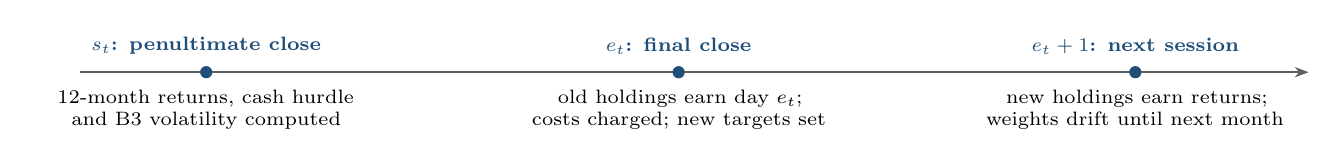
\begin{tikzpicture}[x=1cm,y=1cm,font=\scriptsize]
\draw[-{Stealth[length=5pt]},muted,line width=0.6pt] (0,0) -- (15.6,0);
\foreach \x/\l/\t in {1.6/{$s_t$: penultimate close}/{12-month returns, cash hurdle and B3 volatility computed},7.6/{$e_t$: final close}/{old holdings earn day $e_t$; costs charged; new targets set},13.4/{$e_t+1$: next session}/{new holdings earn returns; weights drift until next month}}{
  \fill[accent] (\x,0) circle (2.2pt);
  \node[above=3pt,text=accent,font=\scriptsize\bfseries] at (\x,0) {\l};
  \node[below=3pt,align=center,text width=4.3cm] at (\x,0) {\t};}
\end{tikzpicture}
\end{center}

\vskip0.05cm
\begin{itemize}\itemsep1pt
\item 12-month signals plus a 126-day volatility history give a common first execution on 2007-08-31 for every ETF strategy and benchmark.
\item One full session separates the signal from the trade, so no decision uses same-day information.
\item Current data vintages may revise history, and the ETF universe was chosen with hindsight; both are standard backtest caveats.
\end{itemize}
\src{Sources: \texttt{outputs/tables/data\_coverage.csv}; \texttt{data/manifests/inputs.json}; \texttt{research/data\_quality.md}.}
\end{frame}

% ------------------------------------------------------------------ 5 ------
\begin{frame}[t]{Portfolio construction: B0, B1 and B2}
\small
Universe $\mathcal{U}=\{\text{SPY, EFA, EEM, IEF, TLT, GLD, DBC, VNQ}\}$; $P_i$ = adjusted close; $s_t$ = penultimate trading day of month $t$.
\vskip0.1cm
\begin{columns}[T,onlytextwidth]
\begin{column}{0.56\textwidth}
\textbf{Signals at $s_t$}
\begin{align*}
M_{i,t} &= \frac{P_i(s_t)}{P_i(s_{t-12})}-1, \\
C_t &= \prod_{d\in(s_{t-12},\,s_t]}(1+\mathrm{RF}_d)-1 .
\end{align*}
$C_t$ spans exactly the signal window. Rank $R_{i,t}$ by descending $M_{i,t}$; ties alphabetical.

\vskip0.15cm
\textbf{Targets executed at $e_t$}
\begin{align*}
w^{B0}_{i,t} &= \tfrac18, \\
w^{B1}_{i,t} &= \tfrac13\,\mathbf{1}[R_{i,t}\le 3], \\
w^{B2}_{i,t} &= \tfrac13\,\mathbf{1}[R_{i,t}\le 3]\;\mathbf{1}[M_{i,t}>C_t], \\
w^{\text{cash}}_{t} &= 1-\textstyle\sum_i w_{i,t}.
\end{align*}
\end{column}
\begin{column}{0.40\textwidth}
\footnotesize
\begin{itemize}\itemsep3pt
\item \textbf{B0}: equal weight, reset monthly.
\item \textbf{B1}: three fixed one-third slots for the top three ETFs.
\item \textbf{B2}: a slot that fails the cash hurdle stays in cash. No refill from rank 4 and no renormalization, so the filter genuinely reduces risk.
\item Monthly snapshots; the latest month is included.
\item Benchmarks: 60/40 = 60\% SPY, 40\% IEF reset monthly; SPY bought and held.
\end{itemize}
\vskip0.1cm
{\scriptsize\color{muted}Every decision is logged in \texttt{outputs/audits/etf\_signals.csv} (lookback dates, $M_{i,t}$, $C_t$, targets).}
\end{column}
\end{columns}
\end{frame}

% ------------------------------------------------------------------ 6 ------
\begin{frame}[t]{B3 risk control: exposure scales down automatically when volatility rises}
\begin{columns}[T,onlytextwidth]
\begin{column}{0.53\textwidth}
\small
Let $x_d$ = daily gross B2 return minus RF, from B2's realized history. At $s_t$:
\begin{align*}
\hat\sigma_t &= \sqrt{252}\;\operatorname{sd}\big(x_{d-125},\dots,x_{d}\big),\quad d=s_t,\\
q_t &= \min\!\Big(1,\;\frac{0.10}{\max(\hat\sigma_t,\,0.05)}\Big),\\
w^{B3}_{i,t} &= q_t\,w^{B2}_{i,t},\qquad w^{\text{cash}} = 1-q_t\textstyle\sum_i w^{B2}_{i,t}.
\end{align*}
\footnotesize
\begin{itemize}\itemsep2pt
\item 126 daily observations, sample standard deviation.
\item $q_t\le 1$: the cap only reduces risk and never adds leverage.
\item On average B3 was \BthreeInvested{} invested, holding \BthreeCash{} in cash.
\end{itemize}
\end{column}
\begin{column}{0.43\textwidth}
\footnotesize
\textbf{Worked example (illustrative)}
\vskip0.1cm
Top-three signals 12\%, 8\%, 1\%; matched cash 2\% $\Rightarrow$ two slots pass. With $\hat\sigma_t=16\%$, $q_t=0.10/0.16=0.625$.
\vskip0.15cm
\begin{tabular}{@{}lrrr@{}}
\toprule
Slot & B1 & B2 & B3 \\
\midrule
Rank 1 (12\%) & 33.33\% & 33.33\% & 20.83\% \\
Rank 2 (8\%) & 33.33\% & 33.33\% & 20.83\% \\
Rank 3 (1\%) & 33.33\% & 0.00\% & 0.00\% \\
\rowcolor{accentlight} Cash & 0.00\% & 33.33\% & 58.33\% \\
\bottomrule
\end{tabular}
\vskip0.12cm
B3 cash = failed slot (33.33\%) + scaling cut $(1-0.625)\times 66.67\%=25.00\%$.
\end{column}
\end{columns}
\src{Historical $q_t$ and $\hat\sigma_t$ per rebalance: \texttt{outputs/audits/etf\_risk\_sizing.csv}.}
\end{frame}

% ------------------------------------------------------------------ 7 ------
\begin{frame}[t]{Results: B3 has the shallowest drawdown and the best return per unit of drawdown}
\footnotesize
\begin{tabular*}{\textwidth}{@{\extracolsep{\fill}}llrrrrrr@{}}
\toprule
Code & Strategy & CAGR & Vol & Sharpe & Max daily DD & Worst month & CAGR/MDD \\
\midrule
\tabinput{generated/tab_main.tex}
\bottomrule
\end{tabular*}

\vskip0.3cm
\small
\begin{itemize}\itemsep2pt
\item \textbf{Each step adds value.} Relative selection lifts CAGR from \BzeroCAGR{} to \BoneCAGR{} and cuts the worst drawdown from \BzeroMDD{} to \BoneMDD. The volatility cap then takes it to \BthreeMDD, the clearest single improvement.
\item \textbf{Versus 60/40:} \DDReduction\% shallower worst drawdown and a smaller worst month, for 1.3 points less annual return. 60/40 keeps a higher Sharpe; B3 is built for investors who rank drawdown control first.
\item The cash hurdle (B2) contributes little to the worst drawdown in this sample; the cap does the heavy lifting.
\end{itemize}
\src{Identical dates for all rows: 2007-08-31 to 2026-08-31, net of 10 bps per traded risky dollar. CAGR/MDD = CAGR $\div$ |max daily drawdown|. Source: \texttt{outputs/tables/performance.csv}.}
\end{frame}

% ------------------------------------------------------------------ 8 ------
\begin{frame}[t]{B3 compounds steadily while avoiding the deep troughs of 60/40 and equities}
\vskip-0.1cm
\begin{center}
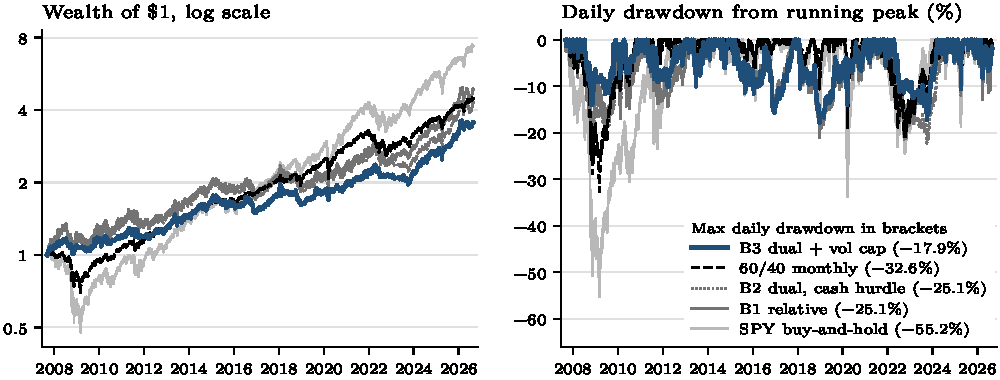
\includegraphics[width=\textwidth]{figures/fig_B_wealth_drawdown.pdf}
\end{center}
\vskip-0.25cm
\src{2007-08-31 (first return 2007-09-04) to 2026-08-31; net of 10 bps per traded risky dollar; drawdown peaks include initial capital. Daily NAV from \texttt{outputs/tables/*\_daily.csv}. B0 not shown (max DD \BzeroMDD).}
\end{frame}

% ------------------------------------------------------------------ 9 ------
\begin{frame}[t]{Consistency: B3 limited losses in both crisis periods and led over 2020--2026}
\footnotesize
\begin{tabular*}{\textwidth}{@{\extracolsep{\fill}}lrrrrrr@{}}
\toprule
 & \multicolumn{3}{c}{B3 vol-capped dual momentum} & \multicolumn{3}{c}{Monthly 60/40} \\
\cmidrule(lr){2-4}\cmidrule(l){5-7}
Period & CAGR & Sharpe & Max daily DD & CAGR & Sharpe & Max daily DD \\
\midrule
\tabinput{generated/tab_sub.tex}
\bottomrule
\end{tabular*}

\vskip0.25cm
\begin{columns}[T,onlytextwidth]
\begin{column}{0.56\textwidth}
\scriptsize
\begin{tabular}{@{}lrrr@{}}
\toprule
Stress measure & B3 & 60/40 & SPY \\
\midrule
\tabinput{generated/tab_stress.tex}
\bottomrule
\end{tabular}
\end{column}
\begin{column}{0.40\textwidth}
\scriptsize
\begin{itemize}\itemsep2pt
\item Smaller drawdowns than 60/40 in 2007--2013 and 2020--2026. In calm 2014--2019 markets, 60/40 did better.
\item 2020--2026: higher return \emph{and} Sharpe than 60/40. These years were reviewed during research, so we treat them as supporting, not out-of-sample, evidence.
\item B3 lags in strong rallies (2020); that is the price of protection.
\end{itemize}
\end{column}
\end{columns}
\src{Paired block bootstrap (6-month blocks, 1{,}000 draws): B3$-$60/40 Sharpe difference \BootSixtyDiff, 95\% interval [\BootSixtyLo, \BootSixtyHi]; the case rests on drawdown, not Sharpe. Sources: \texttt{performance.csv}, \texttt{stress\_periods.csv}, \texttt{bootstrap.csv}.}
\end{frame}

% ------------------------------------------------------------------ 10 -----
\begin{frame}[t]{Robustness: drawdown control holds across costs, timing and breadth}
\begin{columns}[T,onlytextwidth]
\begin{column}{0.60\textwidth}
\footnotesize
\begin{tabular}{@{}lrrrr@{}}
\toprule
B3 variant (one change) & CAGR & $\Delta$ pp & Sharpe & Max DD \\
\midrule
\tabinput{generated/tab_sens.tex}
\bottomrule
\end{tabular}
\end{column}
\begin{column}{0.36\textwidth}
\footnotesize
\begin{itemize}\itemsep3pt
\item Max drawdown stays between $-$14.3\% and $-$24.7\% in every variant.
\item Trading one session later changes almost nothing; even 50 bps costs leave CAGR at 5.2\%.
\item Known dependencies: gold (GLD) diversification and including the latest month.
\item The 9-month signal tested better, but we keep the pre-specified 12-month rule to avoid fitting to history.
\end{itemize}
\end{column}
\end{columns}
\src{Common sensitivity sample 2007-10-31 to 2026-08-31 (needed for the skip-month warm-up), so the first row differs from the headline. Source: \texttt{outputs/tables/sensitivities.csv}; all 84 evaluated rows in \texttt{variant\_ledger.csv}.}
\end{frame}

% ------------------------------------------------------------------ 11 -----
\begin{frame}[t]{Implementation: liquid ETFs, low costs and a staged mandate}
\begin{columns}[T,onlytextwidth]
\begin{column}{0.45\textwidth}
\small
\textbf{Costs}
\footnotesize
\begin{itemize}\itemsep2pt
\item One rebalance a month; turnover \BthreeTurn$\times$ a year (buys + sells).
\item At 10 bps per traded dollar, about \BthreeCostAllowance\% a year; gross CAGR \BthreeGrossCAGR{} vs net \BthreeCAGR.
\item ETF expense ratios are already inside the returns. Even at 50 bps, B3 keeps its drawdown control (slide 10).
\end{itemize}
\vskip0.1cm
\small\textbf{Mandate path}
\footnotesize
\begin{enumerate}\itemsep1pt
\item \textbf{\$1m launch}: every historical trade below 2\% of average daily volume.
\item \textbf{\$10m}: after independent data checks and measured closing-auction costs, with DBC orders sized or split as needed.
\end{enumerate}
\end{column}
\begin{column}{0.51\textwidth}
\small
\textbf{Trade size relative to ADV20, B3}
\vskip0.05cm
\scriptsize
\begin{tabular*}{\linewidth}{@{\extracolsep{\fill}}lrrrrr@{}}
\toprule
 & \$1m & \multicolumn{4}{c}{\$10m scenario} \\
\cmidrule(lr){2-2}\cmidrule(l){3-6}
ETF & Max & Max & p95 & Trades & $>$5\% \\
\midrule
\tabinput{generated/tab_cap.tex}
\bottomrule
\end{tabular*}
\vskip0.15cm
\footnotesize
SPY, EEM, GLD and EFA never exceed 1\% of ADV20 even at \$10m. The constraint is DBC, which peaks at \hl{\DBCtenMax} at \$10m: the reason the mandate is staged.
\end{column}
\end{columns}
\src{Participation = AUM $\times$ NAV $\times |\Delta w|$ / 20-day average dollar volume to the prior signal close; all-day volume, not closing-auction volume. Sources: \texttt{capacity\_summary.csv}, \texttt{capacity\_active\_trades\_summary.csv}.}
\end{frame}

% ------------------------------------------------------------------ 12 -----
\begin{frame}[t]{Investment proposal: who it is for, the risks, and next steps}
\footnotesize
\begin{columns}[T,onlytextwidth]
\begin{column}{0.485\textwidth}
\small\textbf{\color{accent}Why allocate to B3}
\footnotesize
\begin{itemize}\itemsep2pt
\item \textbf{Drawdown control}: \BthreeMDD{} worst drawdown vs \SixtyMDD{} for 60/40 and \BoneMDD{} for relative momentum.
\item \textbf{Diversifies stock--bond risk}: \BthreeYtwentytwo{} in 2022 vs \SixtyYtwentytwo{} for 60/40.
\item \textbf{Transparent}: published rules, liquid ETFs, every signal, trade and NAV auditable; no leverage, no shorting.
\end{itemize}
\vskip0.1cm
\small\textbf{\color{accent}Suited to}\par
\footnotesize
Allocators who value smaller losses over maximum return and can accept periods of lagging in strong rallies.
\end{column}
\begin{column}{0.485\textwidth}
\small\textbf{\color{accent}Key risks and mitigants}
\vskip0.05cm
\scriptsize
\begin{tabular}{@{}>{\raggedright\arraybackslash}p{2.6cm}>{\raggedright\arraybackslash}p{4.3cm}@{}}
\toprule
Risk & Mitigant \\
\midrule
Fast reversals, whipsaw & Monthly rebalancing; volatility cap \\
Lags in sharp rallies & Disclosed: 2020 \BthreeYtwenty{} vs 60/40 \SixtyYtwenty \\
Backtest overfitting & Rules frozen in advance; 9-month variant not adopted \\
Capacity in DBC & Staged mandate from \$1m \\
\bottomrule
\end{tabular}
\vskip0.15cm
\small\textbf{\color{accent}Next steps}
\footnotesize
\begin{enumerate}\itemsep0pt
\item Independent reconciliation of prices and distributions (e.g., CRSP).
\item Measure closing-auction costs; begin time-stamped paper trading.
\item Launch the \$1m mandate; review for scale-up to \$10m.
\end{enumerate}
\end{column}
\end{columns}
\src{Backtested, net of modeled costs; past performance does not guarantee future results. Sources: \texttt{performance.csv}, \texttt{stress\_periods.csv}.}
\end{frame}

\appendix
\begin{frame}[t]{Appendix contents}
\small
\begin{columns}[T,onlytextwidth]
\begin{column}{0.48\textwidth}
\textbf{A: factor research (synthetic gross)}
\begin{enumerate}
\item[\color{accent}1.] A0--A3 construction and conventions
\item[\color{accent}2.] A results and diagnostics
\item[\color{accent}3.] A wealth and drawdown
\end{enumerate}
\vskip0.2cm
\textbf{Methods and precision}
\begin{enumerate}
\item[\color{accent}4.] Trading, cost and metric conventions
\item[\color{accent}5.] B3 exposure management
\item[\color{accent}6.] Five-decimal results table
\end{enumerate}
\end{column}
\begin{column}{0.48\textwidth}
\textbf{Sources}
\begin{enumerate}
\item[\color{accent}7.] References
\item[\color{accent}8.] Data provenance and reproducibility
\end{enumerate}
\vskip0.3cm
\footnotesize\color{muted}
A results are synthetic, gross and dated 1990-01-31 to 2026-08-31. They are shown for research context and are not comparable with the ETF results in the main deck.
\end{column}
\end{columns}
\end{frame}

% ------------------------------------------------------------------ A1 -----
\begin{frame}[t]{Appendix 1. Factor overlay: A0--A3 construction}
\begin{columns}[T,onlytextwidth]
\begin{column}{0.53\textwidth}
\small
Daily synthetic capital return, with $m_d$ = daily French Mom (already an excess spread) and $f_d$ = RF:
\[
r_d = f_d + a_{t}\,m_d - \text{cost}_d .
\]
At the penultimate close $s_t$:
\begin{align*}
\sigma^{\text{Mom}}_t &= \sqrt{252}\,\operatorname{sd}(\text{last 126 } m_d),\\
a^{\text{vol}}_t &= \min\!\Big(1.5,\;\frac{0.10}{\max(\sigma^{\text{Mom}}_t,0.05)}\Big),\\
\text{Bear}_t &= \mathbf{1}\big[\mathrm{TR}^{\text{mkt}}(s_t)/\mathrm{TR}^{\text{mkt}}(s_{t-24})<1\big],\\
\text{HighVol}_t &= \mathbf{1}[\mathrm{VIX}(s_t)>25],\\
g_t &= 1,\ 0.5,\ 0 \ \text{for 0, 1, 2 active flags}.
\end{align*}
\end{column}
\begin{column}{0.43\textwidth}
\footnotesize
\begin{tabular}{@{}lll@{}}
\toprule
Code & Exposure $a_t$ & Role \\
\midrule
A0 & 1 & Static factor \\
A1 & $a^{\text{vol}}_t$ & Volatility scaling \\
A2 & $g_t$ & Bear/VIX regime \\
A3 & $a^{\text{vol}}_t\,g_t$ & Combined \\
\bottomrule
\end{tabular}
\vskip0.2cm
\begin{itemize}\itemsep2pt
\item Exposure held until the next monthly execution. RF is not subtracted twice.
\item One factor unit $\approx$ \$1 long + \$1 short per \$ of capital; the 1.5 cap allows gross notional up to $3\times$.
\item The bear/VIX rule is a heuristic motivated by panic-state evidence \rcite{DM16, pp.\,226--227; KW15, pp.\,59--60}; it is not D\&M's conditional mean--variance strategy.
\item Gross. Illustrative charges ($2|\Delta a|\times$cost, annual drags) omit trading inside Mom and borrow.
\end{itemize}
\end{column}
\end{columns}
\src{Execution 1990-01-31, first return 1990-02-01, end 2026-08-31. Monthly exposure decisions in \texttt{outputs/audits/factor\_decisions.csv}.}
\end{frame}

% ------------------------------------------------------------------ A2 -----
\begin{frame}[t]{Appendix 2. Factor results (synthetic, gross of stock-level costs)}
\footnotesize
\begin{tabular*}{\textwidth}{@{\extracolsep{\fill}}llrrrrrr@{}}
\toprule
Code & Strategy & CAGR & Ann.\ vol & Sharpe & Max daily DD & Avg exposure & Exposure turnover/yr \\
\midrule
\tabinput{generated/tab_A.tex}
\bottomrule
\end{tabular*}

\vskip0.3cm
\begin{columns}[T,onlytextwidth]
\begin{column}{0.56\textwidth}
\scriptsize
\begin{tabular}{@{}lrrrrrr@{}}
\toprule
 & \multicolumn{3}{c}{A0 static} & \multicolumn{3}{c}{A3 combined} \\
\cmidrule(lr){2-4}\cmidrule(l){5-7}
Period & CAGR & Sharpe & DD & CAGR & Sharpe & DD \\
\midrule
\tabinput{generated/tab_A_sub.tex}
\bottomrule
\end{tabular}
\end{column}
\begin{column}{0.41\textwidth}
\scriptsize
\begin{itemize}\itemsep2pt
\item Both flags active at 6.8\% of monthly decisions; any flag in 25\%; the 1.5 cap binds in 22.5\%.
\item March--May 2009: A0 lost 45.6\%; A2/A3 had zero factor exposure. That is de-risking, not a hedge.
\item A3$-$A0 Sharpe difference 0.501, bootstrap interval [0.208, 0.760], before any missing costs.
\end{itemize}
\end{column}
\end{columns}
\src{Basis: cash + factor exposure, gross; underlying stock turnover, financing and borrow costs not measured. Sources: \texttt{performance.csv} (prototype A), \texttt{factor\_sizing\_diagnostics.csv}, \texttt{stress\_periods.csv}, \texttt{bootstrap.csv}.}
\end{frame}

% ------------------------------------------------------------------ A3 -----
\begin{frame}[t]{Appendix 3. Factor wealth and drawdown (synthetic gross, 1990--2026)}
\vskip-0.1cm
\begin{center}
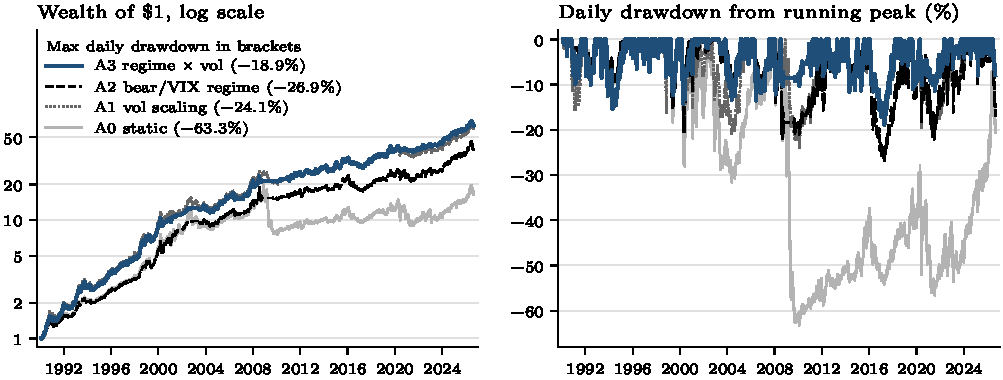
\includegraphics[width=0.90\textwidth]{figures/fig_A_wealth_drawdown.pdf}
\end{center}
\vskip-0.25cm
\src{Daily files \texttt{outputs/tables/A\{0,1,2,3\}\_daily.csv}. Execution 1990-01-31 (first return 1990-02-01) to 2026-08-31. Synthetic cash + daily French Mom exposure, \textbf{gross}. Peaks include initial \$1. Historical crash protection motivates research; it does not establish implementability.}
\end{frame}

% ------------------------------------------------------------------ A4 -----
\begin{frame}[t]{Appendix 4. Trading, cost and metric conventions}
\begin{columns}[T,onlytextwidth]
\begin{column}{0.50\textwidth}
\small\textbf{Daily drift and rebalancing}
\footnotesize
\begin{align*}
R^{\text{gross}}_d &= \textstyle\sum_i w_{i,d-1}\,r_{i,d} + w^{\text{cash}}_{d-1}\mathrm{RF}_d,\\
\tilde w_{i,d} &= w_{i,d-1}(1+r_{i,d})/(1+R^{\text{gross}}_d),\\
T_t &= \textstyle\sum_{i\neq\text{cash}} \big|w^{*}_{i,t}-\tilde w_{i,e_t}\big|,\\
V^{\text{after}} &= V^{\text{before}}(1+R^{\text{gross}}_{e_t})(1-c\,T_t),\quad c=0.001 .
\end{align*}
Old holdings earn the execution-day return, then the cost is charged and post-cost NAV is allocated to targets. A full switch has $T=2$ (20 bps). Initial purchases are charged.

\vskip0.1cm
\textit{Example:} 50/50 in X/Y, X $+10\%$ $\Rightarrow$ weights 52.38/47.62\%; moving to 100\% Y gives $T=1.0476$, cost 10.48 bps.
\end{column}
\begin{column}{0.46\textwidth}
\small\textbf{Metrics}
\footnotesize
\begin{align*}
\text{CAGR} &= V_{\text{end}}^{365.25/\text{days}}-1 \quad(\text{from execution date}),\\
\text{Sharpe} &= \sqrt{12}\,\overline{x}/\operatorname{sd}(x),\\
\text{MDD} &= \min_t\big(V_t/\max_{s\le t}V_s-1\big),\ V_0=1 .
\end{align*}
\begin{itemize}\itemsep2pt
\item $x$ = compounded monthly capital return minus compounded daily RF; sample s.d.
\item Annual vol $=\sqrt{12}\,\operatorname{sd}$ of monthly returns.
\item The initial cost stays in daily NAV and enters the first full month for monthly statistics.
\item Daily and month-end drawdowns are separate fields; the deck reports daily.
\item Adj Close includes distributions; nothing added twice.
\end{itemize}
\end{column}
\end{columns}
\src{Independent reconciliation of trades, weights and NAV: \texttt{outputs/audits/independent\_accounting\_checks.csv}.}
\end{frame}

% ------------------------------------------------------------------ A5 -----
\begin{frame}[t]{Appendix 5. B3 exposure management over time}
\vskip-0.05cm
\begin{center}
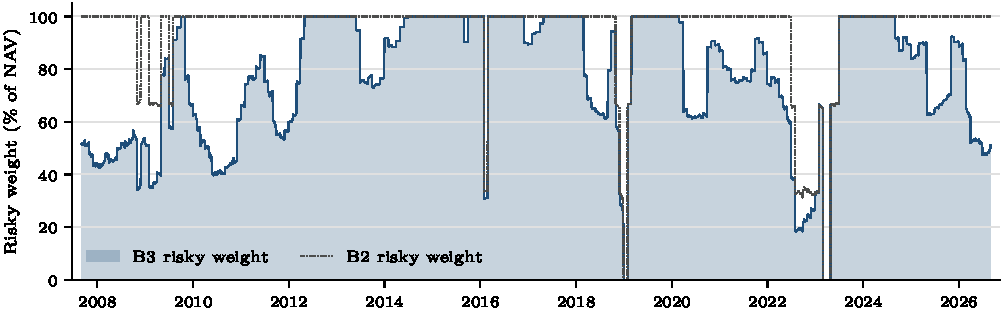
\includegraphics[width=0.92\textwidth]{figures/fig_B3_exposure.pdf}
\end{center}
\vskip-0.15cm
\small
\begin{itemize}\itemsep1pt
\item Average cash: B3 \BthreeCash{} vs B2 \BtwoCash. The cap bound most persistently in 2007--2011; the deepest cash periods (late 2018--2019, 2022--23) came mainly from slots failing the cash hurdle.
\item Exposure falls in turbulent markets and returns toward 100\% in steady trends. Lower exposure in high-volatility periods is the main source of B3's smaller drawdowns.
\end{itemize}
\src{End-of-day weights from \texttt{outputs/tables/B3\_daily.csv} and \texttt{B2\_daily.csv} (risky weight = 1 $-$ cash weight). Execution 2007-08-31 to 2026-08-31.}
\end{frame}

% ------------------------------------------------------------------ A6 -----
\begin{frame}[t]{Appendix 6. Five-decimal results (decimals, not percentages)}
\scriptsize
\begin{tabular*}{\textwidth}{@{\extracolsep{\fill}}lllrrrrrr@{}}
\toprule
Code & Start & Basis & CAGR & Ann.\ vol & Sharpe & Sortino & Max daily DD & Turnover/yr \\
\midrule
\tabinput{generated/tab_precise.tex}
\bottomrule
\end{tabular*}
\vskip0.25cm
\footnotesize
Values are decimals: 0.06891 means 6.891\%. All B rows end 2026-08-31 with the same execution start; A rows are synthetic gross with a different start and are not comparable with B. Cash has no Sharpe or Sortino because its excess return is zero by construction. For A, turnover is change in factor exposure, not stock turnover.
\src{Source: \texttt{outputs/tables/performance.csv}, sample \texttt{full}; rounded from full precision by \texttt{scripts/build\_assets.py}.}
\end{frame}

% ------------------------------------------------------------------ A8 -----
\begin{frame}[t]{Appendix 7. References}
\footnotesize
\begin{itemize}\itemsep3pt
\item[] Venetoulias, A. (Fall 2026). \emph{B9339 Lectures 3--5: Momentum}. Columbia Business School. Slides 4--7, 17--23, 42--49, 65--88. \rcite{Lecture}
\item[] Daniel, K., \& Moskowitz, T. J. (2016). Momentum crashes. \emph{Journal of Financial Economics}, 122(2), 221--247. \rcite{DM16}
\item[] Asness, C., Frazzini, A., Israel, R., \& Moskowitz, T. J. (2014). Fact, fiction and momentum investing. \emph{Journal of Portfolio Management}, 40(5), 75--92. \rcite{AFIM14}
\item[] Kolanovic, M., \& Wei, Z. (April 2015). \emph{Momentum Strategies Across Asset Classes: Risk Factor Approach to Trend Following}. J.P. Morgan. pp.\ 19--20, 59--60. \rcite{KW15}
\item[] Baltas, A.-N., \& Kosowski, R. (supplied version dated January 2013). \emph{Momentum Strategies in Futures Markets and Trend-Following Funds}. Working paper, section 3. \rcite{BK13}
\end{itemize}
\vskip0.2cm
\textbf{Data providers}: Kenneth R.\ French Data Library (daily and monthly Mom, Fama--French factors, RF); Cboe VIX historical closes; Yahoo Finance via yfinance 1.7.0. Methodology URLs and access dates are in \texttt{research/source\_map.md}.
\src{Page and slide locations follow \texttt{research/source\_map.md} of the original package. Readings support motivation and method; they do not supply this portfolio's results.}
\end{frame}

% ------------------------------------------------------------------ A9 -----
\begin{frame}[t]{Appendix 8. Data provenance and reproducibility}
\footnotesize
\begin{columns}[T,onlytextwidth]
\begin{column}{0.48\textwidth}
\textbf{Original research package} (unchanged)
\begin{itemize}\itemsep1pt
\item \texttt{data/raw}, \texttt{data/manifests}: snapshots, URLs, timestamps, SHA-256.
\item \texttt{config/base.yaml}, \texttt{research/freeze.json}: frozen rules.
\item \texttt{src/}: shared backtest code; \texttt{notebooks/}: executed walk-throughs.
\item \texttt{outputs/tables}: canonical returns and metrics; \texttt{outputs/audits}: signals, targets, trades, holdings, clean-run hashes.
\end{itemize}
\vskip0.1cm
Reproduce (Python 3.12, cached data, offline):\\
package command-line interface, \texttt{run -{}-offline}\\
\texttt{python scripts/clean\_reproduce.py}
\end{column}
\begin{column}{0.48\textwidth}
\textbf{Presentation build}
\begin{itemize}\itemsep1pt
\item \texttt{scripts/build\_assets.py} reads only \texttt{outputs/tables/*.csv}, writes \texttt{generated/*.tex} and \texttt{figures/*.pdf}, and asserts the headline values and chart drawdowns against \texttt{performance.csv}.
\item Build: \texttt{python3 scripts/build\_assets.py}, then \texttt{pdflatex} twice.
\end{itemize}
\vskip0.1cm
\textbf{Data caveats}: public caches for personal academic use; current vintages may be revised; universe chosen retrospectively.
\end{column}
\end{columns}
\end{frame}

\end{document}
